% !TEX root = main_hessenberg.tex
\documentclass[11pt]{article}

\usepackage[a4paper,margin=1in]{geometry}
\usepackage{amsmath,amssymb,amsthm,mathtools}
\usepackage{enumitem}
\usepackage{hyperref}
\usepackage{tikz}
\usepackage{listings}
\usepackage{xcolor}
\usepackage{booktabs}
\usepackage{tabularx}
\usepackage[utf8]{inputenc}
\usepackage{placeins}
\usetikzlibrary{matrix,backgrounds,fit,positioning,arrows.meta,calc}

% --- Schmitt-style human/AI attribution (for appendix) ---
\usepackage[normalem]{ulem}
\usepackage[breakable,skins]{tcolorbox}

\definecolor{humancolor}{RGB}{0, 102, 204}
\definecolor{aicolor}{RGB}{180, 90, 50}

\newlength{\marginbarwidth}
\setlength{\marginbarwidth}{2pt}
\newlength{\marginbarsep}
\setlength{\marginbarsep}{6pt}

\newtcolorbox{humanparagraph}{%
  enhanced, breakable, blanker,
  borderline west={\marginbarwidth}{-\marginbarsep}{humancolor},
  left=0pt, right=0pt, top=2pt, bottom=2pt,
  before skip=0.5\baselineskip, after skip=0.5\baselineskip,
  overlay unbroken and first={
    \node[humancolor, font=\tiny\scshape, rotate=90, anchor=north]
      at ([xshift=-\marginbarsep-\marginbarwidth/2-12pt, yshift=-13pt]frame.north west) {Human};
  }
}

\newtcolorbox{aiparagraph}{%
  enhanced, breakable, blanker,
  borderline west={\marginbarwidth}{-\marginbarsep}{aicolor},
  left=0pt, right=0pt, top=2pt, bottom=2pt,
  before skip=0.5\baselineskip, after skip=0.5\baselineskip,
  overlay unbroken and first={
    \node[aicolor, font=\tiny\scshape, rotate=90, anchor=north]
      at ([xshift=-\marginbarsep-\marginbarwidth/2-12pt, yshift=-5pt]frame.north west) {AI};
  }
}

% --- Typography ---
\newcommand{\defeq}{\coloneqq}

% --- Code listing style ---
\definecolor{codegreen}{rgb}{0,0.6,0}
\definecolor{codegray}{rgb}{0.5,0.5,0.5}
\definecolor{codepurple}{rgb}{0.58,0,0.82}
\definecolor{backcolour}{rgb}{0.97,0.97,0.95}
\definecolor{kwblue}{RGB}{0,112,192}
\definecolor{typorange}{RGB}{180,90,50}

\lstdefinelanguage{Lean}{
  morekeywords={
    import, open, namespace, end, section, variable, universe,
    theorem, lemma, def, abbrev, instance, structure, class, example,
    axiom, opaque, mutual, where, noncomputable, set_option,
    fun, let, have, show, by, do, match, with, if, then, else,
    return, in, from, inductive
  },
  morekeywords=[2]{
    set, obtain, refine, exact, apply, intro, intros, rintro, rcases,
    induction, cases, constructor, calc, simp, ring, linarith, omega,
    rfl, decide, trivial, sorry, admit, push_cast, norm_num, positivity,
    field_simp, ext, by_contra, rw, rewrite, change, subst, unfold,
    assumption, dsimp, simp_all
  },
  morekeywords=[3]{
    True, False, And, Or, Not, Eq, Iff, Prop, Type, Sort,
    forall, exists, Fin, Nat, Real, Matrix, Finset, Equiv, Perm, List, Bool
  },
  sensitive=true,
  morecomment=[l]{--},
  morecomment=[s]{/-}{-/},
  morestring=[b]"
}
\definecolor{leankw}{HTML}{0033B3}      % top-level keywords (blue)
\definecolor{leantactic}{HTML}{8B008B}  % tactics (purple)
\definecolor{leanbuiltin}{HTML}{1F7A6F} % built-in / Prop / forall (teal)
\definecolor{leancomment}{HTML}{6A737D} % comments (gray)
\definecolor{leanstring}{HTML}{C41A16}  % strings (red)
\lstset{
  language=Lean,
  basicstyle=\footnotesize\ttfamily,
  keywordstyle=\color{leankw}\bfseries,
  keywordstyle=[2]\color{leantactic},
  keywordstyle=[3]\color{leanbuiltin},
  commentstyle=\color{leancomment}\itshape,
  stringstyle=\color{leanstring},
  breaklines=true,
  columns=fullflexible,
  keepspaces=true,
  frame=single,
  framesep=4pt,
  rulecolor=\color{black!30},
  showstringspaces=false,
  aboveskip=6pt,
  belowskip=6pt,
  extendedchars=true,
  inputencoding=utf8,
  literate=
    {->}{{$\to$}}1
    {=>}{{$\Rightarrow$}}1
    {<->}{{$\leftrightarrow$}}1
    {!=}{{$\neq$}}1
    {<=}{{$\le$}}1
    {>=}{{$\ge$}}1
    {/\\}{{$\wedge$}}1
    {\\/}{{$\vee$}}1
    {forall}{{$\forall$}}1
    {exists}{{$\exists$}}1
    {lambda}{{$\lambda$}}1
    {=~=}{{$\cong$}}1
    {∀}{{$\forall$}}1
    {∃}{{$\exists$}}1
    {≤}{{$\le$}}1
    {≥}{{$\ge$}}1
    {≠}{{$\neq$}}1
    {≅}{{$\cong$}}1
    {→}{{$\to$}}1
    {⇒}{{$\Rightarrow$}}1
    {↔}{{$\leftrightarrow$}}1
    {↦}{{$\mapsto$}}1
    {∧}{{$\wedge$}}1
    {∨}{{$\vee$}}1
    {¬}{{$\neg$}}1
    {θ}{{$\theta$}}1
    {α}{{$\alpha$}}1
    {β}{{$\beta$}}1
    {γ}{{$\gamma$}}1
    {δ}{{$\delta$}}1
    {ε}{{$\varepsilon$}}1
    {σ}{{$\sigma$}}1
    {φ}{{$\varphi$}}1
    {ψ}{{$\psi$}}1
    {ω}{{$\omega$}}1
    {Γ}{{$\Gamma$}}1
    {Δ}{{$\Delta$}}1
    {Σ}{{$\Sigma$}}1
    {Π}{{$\Pi$}}1
    {ℕ}{{$\mathbb{N}$}}1
    {ℝ}{{$\mathbb{R}$}}1
    {ℤ}{{$\mathbb{Z}$}}1
    {ℚ}{{$\mathbb{Q}$}}1
    {ℂ}{{$\mathbb{C}$}}1
    {⟨}{{$\langle$}}1
    {⟩}{{$\rangle$}}1
    {⊢}{{$\vdash$}}1
    {⊕}{{$\oplus$}}1
    {⊗}{{$\otimes$}}1
    {∘}{{$\circ$}}1
    {∈}{{$\in$}}1
    {∉}{{$\not\in$}}1
    {⊆}{{$\subseteq$}}1
    {∪}{{$\cup$}}1
    {∩}{{$\cap$}}1
    {∅}{{$\emptyset$}}1
}

% --- Hyperlinks ---
\hypersetup{
    colorlinks=true,
    linkcolor={blue!70!black},
    citecolor={blue!70!black},
    urlcolor={blue!70!black},
    pdfborder={0 0 0},
}

% --- Theorem numbering ---
\newtheorem{theorem}{Theorem}[section]
\newtheorem{proposition}[theorem]{Proposition}
\newtheorem{lemma}[theorem]{Lemma}
\newtheorem{corollary}[theorem]{Corollary}
\theoremstyle{definition}
\newtheorem{definition}[theorem]{Definition}
\newtheorem{example}[theorem]{Example}
\theoremstyle{remark}
\newtheorem{remark}[theorem]{Remark}

% --- Macros ---
\newcommand{\R}{\mathbb{R}}
\newcommand{\N}{\mathbb{N}}
\newcommand{\Id}{I}
\newcommand{\Ind}{\mathbf{1}}


\title{Marshmallow formalization by prompt design}
\author{
 Xinze Li\thanks{Department of Mathematics, University of Toronto}
 \and
 Simone Severini\thanks{Department of Computer Science,
  UCL}
}
\date{\today}

% Lean-link macros (comb-arg style): green checkmark + clickable declaration name.
%   \lean{decl\_name}{File/Path.lean}        -- inline tag
%   \leanmargin{decl\_name}{File/Path.lean}  -- right-flushed [✓ name] after theorem/def label
\newcommand{\leanrepo}{https://github.com/simoneseverini/Digraphs-of-Real-Orthogonal-Upper-Hessenberg-Matrices/blob/main/lean/HessenbergDigraphs}
\definecolor{leangreen}{HTML}{006400}
\newcommand{\lean}[2]{{\normalfont\color{leangreen}%
  \ensuremath{\checkmark}\,\href{\leanrepo/#2}{\texttt{#1}}}}
\newcommand{\leanmargin}[2]{%
  \nopagebreak\hfill{\normalfont\small\color{leangreen}%
    [\ensuremath{\checkmark}\,\href{\leanrepo/#2}{\texttt{#1}}]}\par\nopagebreak
}
\newcommand{\leanmargintwo}[4]{%
  \nopagebreak\hfill{\normalfont\small\color{leangreen}%
    [\ensuremath{\checkmark}\,\href{\leanrepo/#2}{\texttt{#1}},
     \ensuremath{\checkmark}\,\href{\leanrepo/#4}{\texttt{#3}}]}\par\nopagebreak
}
% \leanmarginLean: like \leanmargin but path is relative to lean/ (the
% lake package root), not lean/HessenbergDigraphs/. Used for the
% project's tooling under lean/Util/.
\newcommand{\leanrepoLean}{https://github.com/simoneseverini/Digraphs-of-Real-Orthogonal-Upper-Hessenberg-Matrices/blob/main/lean}
\newcommand{\leanmarginLean}[2]{%
  \nopagebreak\hfill{\normalfont\small\color{leangreen}%
    [\ensuremath{\checkmark}\,\href{\leanrepoLean/#2}{\texttt{#1}}]}\par\nopagebreak
}

\begin{document}
\maketitle

\begin{abstract}
%As AI-assisted Lean formalizations emerge where authors write no code, the human role increasingly shifts toward prompt design and mathematical judgment. In this paradigm, treating the code as the primary artifact requires some methodological discipline. We present a protocol \textcolor{red}{ (“protocol” too strong for a case study?)} that isolates non-mathematical engineering tax from the core content, ensuring formal theorem signatures read exactly as their corresponding paper sentences \textcolor{red}{(We actually trying to make the paper fits the code, rather than make the code fit the paper)}. For a community adapting to AI assistants, this work reminds us of a principle: compilation is not necessarily completion. We validate this approach through a complete, publicly available Lean 4 case study in combinatorial matrix theory.

%\textcolor{red}{\textbf{New Version: }

As AI-assisted Lean formalizations emerge where authors write little or no code, the human role shifts toward prompt design and mathematical judgment. In this paradigm, treating code as the primary mathematical artifact requires some methodological discipline: the standards we hold code to as software (readability, naming, structural discipline) must carry over to it as mathematics. We present an approach with two aims: non-mathematical engineering overhead is separated out so it can be managed on its own, and the prose serves only as an interface to the formal development, which carries the mathematics itself. 
We validate this approach through a mathematical ``marshmallow"—a small but intellectually rewarding problem—by providing a publicly available Lean 4 case study in combinatorial matrix theory.


%Given a real orthogonal upper Hessenberg matrix $Q \in \mathbb{R}^{n \times n}$,
%we study its support digraph $D(Q)$ on the vertex set $[n]$, where an arc
%$i \to j$ exists if and only if $Q_{ij} \neq 0$. Using a canonical factorization
%into adjacent Givens rotations, we derive an explicit closed form for the matrix
%entries, which precisely determines their zero--nonzero pattern. We show that
%$D(Q)$ is weakly connected if and only if $Q$ is unreduced, and in this case
%the digraph is strongly connected, contains a unique directed Hamilton cycle,
%and is completely parameterized by a subset $S \subseteq [n-1]$. By analyzing
%exact vertex degrees and directed distances, we prove that these digraphs
%possess a trivial automorphism group whenever $|S| \ge 2$. This structural
%rigidity enables us to exactly enumerate the isomorphism classes, showing
%there are precisely $2^{n-1} - \lfloor \frac{n-1}{2} \rfloor$ non-isomorphic
%connected support digraphs on $n$ vertices. Finally, we classify the loopless
%connected support digraphs, establishing a bijection with integer subsets
%lacking consecutive elements, and prove they are enumerated by
%$F_{n-1} - \lfloor \frac{n-3}{2} %\rfloor$, where $F_k$ is the $k$-th
%Fibonacci number.

%All results have been completely formalized and machine-verified in the Lean~4 proof assistant, building on the Mathlib library. The entire development compiles with zero \texttt{sorry} and depends only on Lean~4's standard axioms. The formalization was carried out semi-autonomously by an AI agent system, with human-guided strategy for the most challenging proofs.
\end{abstract}

%{\small\tableofcontents}

% =====================================================================

% !TEX root = ../main_hessenberg.tex
\section{Introduction}\label{sec:intro}

AI tools can now produce substantial Lean developments under human prompt
design~\cite{ilin2026semiautonomousvml, avigad2026mathematiciansageai}. This
shifts the practical question of how a formalization is built, and with it, the
methodological question of what a formalization is for. Lean is built on
dependent type theory, in which the Curry--Howard correspondence identifies
proofs with terms and mathematical statements with
types~\cite{deMoura2021Lean4}; in this sense, the formal development of a proof
is the proof itself. The major formalization successes of the last five
years~\cite{lean_liquid, vandoorn2023sphereeversion,
Anderson_Formalization_of_the_2023, becker2025carleson_blueprint,
bolan2025equationaltheoriesprojectadvancing, flt_lean} have been carried out
alongside reflective accounts of the practice of building such
developments~\cite{Avigad2023MathematicsAT, avigad2026mathematiciansageai}.

We report a case study that takes the Curry--Howard correspondence as its
working premise: the formal Lean development is the mathematics, and the prose
only renders it. The premise is not ours; a growing literature examines the
methodological consequences of treating formal developments as designed
mathematical artifacts~\cite{commelin2023abstractionboundariesspecdriven,
baanen2025growing, vandoorn2020maintaining, avigad2024anatomyformalproof,
ilin2026semiautonomousvml}. Our contribution is to set out the practices that
follow when the premise is enforced end to end. A network analysis of
\texttt{Mathlib}~\cite{li2026networkstructuremathlib} shows its structure to be
heavily infrastructural (\emph{e.g.}, coercions and typeclasses) rather than
strictly mathematical; the practices below apply this library-wide distinction
to a single development. We tag every declaration as mathematical content or
\emph{engineering tax}, that is, scaffolding with no mathematical counterpart.
We gather this overhead into a standalone Foundation layer that the
mathematical layer reaches only through clean interfaces. We enforce a naming
discipline under which every declaration reads aloud as a mathematical
statement. Under this arrangement the authors write no code: they steer the
formalization entirely through prompt design and mathematical judgment. The
central principle is as follows:
\begin{center}
\emph{the code must read as mathematics.}
\end{center}

As a case study, we characterize the digraphs of real-orthogonal upper
Hessenberg matrices, a small, self-contained problem that revisits a question
first considered in~\cite{severini2003a}. Nothing in the practices depends on
the problem being small; if anything, keeping engineering tax out of the
mathematical narrative matters more in a large formalization, where the
narrative is easiest to lose. Section~\ref{sec:methodology} sets out the
practices, and Section~\ref{sec:example} presents the case study, with direct
cross-references into the Lean development. The full development is available
\href{https://github.com/simoneseverini/Digraphs-of-Real-Orthogonal-Upper-Hessenberg-Matrices}{on
GitHub}; every theorem and definition below carries a link into its source.

We have also published the mathematics of Section~\ref{sec:example} on
\href{https://www.astrolabe.network/writing/hessenberg-digraphs}{\texttt{astrolabe.network}},
where every statement is cut into a card addressed by a unique hash, and the
relations between cards are themselves nodes, each carrying the semantics of
the relation it stands for. The visualization and the network analyses it
carries follow~\cite{li2026networkstructuremathlib}; the underlying design was
set out in~\cite{li2026astrolabecontentaddressablehypergraphsemantic}. Astrolabe
has since evolved substantially, and this network should be read as a prototype
instance of an evolving publication format rather than a fixed specification.



% !TEX root = ../main_hessenberg.tex
\section{Formalization as the primary artifact}\label{sec:methodology}

\sloppy

In dependent type theory, a Lean formalization is inherently a proof~\cite{deMoura2021Lean4}, requiring no accompanying prose. On this basis, we treat the Lean development as the primary mathematical artifact of this project, and the prose as merely one rendering of it. Because the human contribution shifts from writing code to exercising mathematical judgment and steering the AI, the central object of study of this paper is precisely prompt design. Getting the proof to compile is the starting point of that work, not its endpoint. What distinguishes a primary mathematical artifact from a mere verification record lies entirely past that threshold: it depends on whether the code, in its own form, legibly conveys its mathematical content. Finally, we acknowledge that neither author has a formal software engineering background. We treat AI tools as informal mentors in software practice, working to elevate this project to structural standards we did not initially command, and we expect our execution will still reflect this learning curve.

\medskip
\noindent\textbf{Prompt example --- project bootstrap.}
\begin{quote}\itshape\small
The goal is not just proving the main theorem; it is producing code
whose main theorem signature reads as a literal translation of the paper
sentence. Engineering tax should be separated from mathematical content
and encapsulated in independent modules; every name should carry clear
mathematical semantics. Survey the paper's core mathematical objects;
propose a Foundation-structure design. Output the design only; do
not implement until I confirm.
\end{quote}

%\subsection{Engineering tax: see it, then move it}\label{ssec:tax}

We refer to type-theoretic overhead with no paper analogue as
\emph{engineering tax}. Left unmanaged, this tax sits mixed among
mathematical-layer declarations and muddles the mathematical narrative.
Three forms recur in this project:
\begin{itemize}[leftmargin=2em, itemsep=2pt, topsep=2pt]
\item bound-carrying boilerplate, where anonymous-constructor
  expressions bundle a value together with proofs that it lies in range;
\item index translations, where the formal system's natural index
  types differ from the paper's mathematical indexing conventions;
\item case analyses on small numeric ranges, where boundary cases
  dismissed by the paper in a single sentence require explicit,
  separate handling.
\end{itemize}
A typical instance is the lemma \texttt{cyclic\_shift\_arc\_forward}:
its statement reads like a standard mathematical theorem, while its proof body
spans roughly $80$ lines combining all three forms of overhead. A casual
reading of the code easily overlooks the true density of this burden.

To surface this hidden overhead, we tag every declaration as \texttt{Math}, 
\texttt{Eng}, or \texttt{Mixed}. Because these tags are formatted as docstrings 
above each declaration, they travel inherently with the code:
\begin{lstlisting}
/-! ## Mathematical layer -- paper-side vertex type. A `Vertex n`
    is a label `v ∈ {1, ..., n}` (Sec. 0 of the paper). -/

/-! ## Engineering layer -- Type B bridge: `Vertex n ↔ Fin n`
    (paper 1-indexed ↔ Lean 0-indexed). -/
\end{lstlisting}
We enforce this tagging discipline with a small project-specific linter, 
alongside Mathlib's standard tooling~\cite{The_mathlib_Community_2020} 
(naming, docstrings, style, plus \texttt{shake} for unused imports), 
ensuring that violations surface mechanically.

Engineering tax cannot be eliminated, but its location can be chosen.
We encapsulate it in independent modules so the mathematical layer
interacts with them strictly through clean APIs. This applies Parnas's
information-hiding principle~\cite{Parnas1972} to formalization: each
module hides one engineering concern from the mathematical layer. The
core of this effort is a small Foundation layer of bundled structures,
each encapsulating a paper-side mathematical object as a Lean
type~\cite{Baanen_2022, commelin2023abstractionboundariesspecdriven, pittphilsci13482}.
The layer introduces \texttt{Vertex}, \texttt{ActiveSet},
\texttt{Digraph}, \texttt{OrthogonalHessenberg},
\texttt{UnreducedAngles}, and others---allowing each structure to absorb the
corresponding combination of hypotheses just once. Three further modules
(\texttt{Singleton.Fin}, \texttt{EntryAccess},
\texttt{PartialProduct}) are factored out by thematic content.

Such structural refactors involve large-scale cascades---the largest spanned
$12$ files and roughly $232$ call sites---where the design judgment is
made by humans and the execution is carried out by AI. To illustrate the impact, consider the Bridge theorem signature before the 
structural pass:
\begin{lstlisting}
theorem digraph_model (hn : 2 ≤ n) (θ : Fin (n - 1) → ℝ)
    (hunred : ∀ k, Real.sin (θ k) ≠ 0) :
    ∀ i j : Fin n,
      givensProduct θ i j ≠ 0 ↔ Arc n (activeSet θ) (i.val + 1) (j.val + 1)
\end{lstlisting}
After the structural pass:
\begin{lstlisting}
theorem digraph_model (hn : 2 ≤ n) (θ : UnreducedAngles n) :
    θ.product.supportDigraph = θ.activeSet.digraph
\end{lstlisting}
The engineering tax has not disappeared; it simply now lives within the Foundation
modules. Consequently, the formal Bridge theorem reads exactly as the 
natural-language paper sentence.

\medskip
\noindent\textbf{Prompt example --- abstraction design.}
\begin{quote}\itshape\small
Scan all uses of \texttt{Fin n} that represent paper-side vertices.
Report the count of anonymous-mk constructions, the count of
$0$-indexed-to-$1$-indexed translations, and the most common usage
patterns. From the data, propose a \texttt{Vertex n} structure with
constructors, comparison, neighbouring, and a round-trip API to
\texttt{Fin n}. Output the design only.
\end{quote}

%\subsection{Letting mathematics speak}\label{ssec:speak}

Once the engineering tax is isolated, the mathematical layer can carry
semantics directly: names become clear mathematical statements, symbols
match the paper, and the main theorem signature reads as a literal
translation of its natural-language counterpart.

For naming, we apply a simple heuristic: read the name aloud and check
whether it forms a complete mathematical thought. A name that fails
this test usually signals that the declaration's role has not been fully
resolved---it may be too specific, too abstract, or in the wrong place. 
For instance, \texttt{extended\_diag\_isPlusMinusOne} fails because it 
leaves the subject ambiguous; revised to 
\texttt{boundaryAppended\_diag\_isPlusMinusOne}, it forms a clear sentence. 
This test serves both human and AI readability. Placeholder names like 
\texttt{aux\_lemma\_3} leave the AI with no semantic basis for judgment in 
search and completion, whereas a name that encodes its own statement exposes 
the underlying mathematics directly to the model.

We use the form of the main theorem itself as the project's completion 
criterion: when the apex signature reads exactly as the paper sentence, 
the work is done. A green build is necessary, but not sufficient. Consider the apex theorem immediately after proof completion, before the 
engineering tax has been extracted:
\begin{lstlisting}
theorem classification {n : ℕ} (hn : 2 ≤ n) :
    (∀ S : Finset ℕ, ValidS n S → ∃ θ : Fin (n-1) → ℝ,
        (∀ k, Real.sin (θ k) ≠ 0) ∧ activeSet θ = S) ∧
    (∀ θ : Fin (n-1) → ℝ, (∀ k, Real.sin (θ k) ≠ 0) →
        ∀ i j : Fin n, givensProduct θ i j ≠ 0 ↔
          Arc n (activeSet θ) (i.val + 1) (j.val + 1)) ∧
    (∀ S S' : Finset ℕ, ValidS n S → ValidS n S' →
        2 ≤ S.card → 2 ≤ S'.card → DigraphIso n S S' → S = S')
\end{lstlisting}
Here, engineering overhead sits alongside mathematical content in the
signature, forcing the reader to mentally filter it out. The code is 
mathematically verified, but it has not assumed responsibility for legibility. Contrast this with the signature after the structural pass:
\begin{lstlisting}
theorem classification {n : ℕ} (hn : 2 ≤ n) :
    (∀ S : ActiveSet n, ∃ θ : UnreducedAngles n, θ.activeSet = S) ∧
    (∀ θ : UnreducedAngles n, θ.product.supportDigraph = θ.activeSet.digraph) ∧
    (∀ S S' : ActiveSet n, 2 ≤ S.elements.card → 2 ≤ S'.elements.card →
        S.digraph ≅ S'.digraph → S = S') :=
  ⟨completeness, digraph_model hn, fun S S' => rigid S S' hn⟩
\end{lstlisting}
Every conceptual object in the signature is now packaged inside its own
structure. The entire declaration reads as a direct translation of
Theorem~\ref{thm:classification}: for $n \ge 2$, every active set
arises from some unreduced angle vector; the support digraph of the
Givens product equals the one given by the active set; and for
$|S|, |S'| \ge 2$, digraph isomorphism implies $S = S'$.

Both signatures encode identical mathematical content; the difference
lies entirely in whether the code assumes responsibility for its own legibility. 
Only when the formal development is treated as the primary mathematical 
artifact can this standard be posed and met.

\medskip
\noindent\textbf{Prompt example---naming review.}
\begin{quote}\itshape\small
Apply the natural-language reading test to every helper in this file.
For each name that fails, identify the failure mode (missing subject,
placeholder word, unexpanded abbreviation) and propose a revised name
that states what the object is, what it is built from, and what
property it has. Report the rename list; confirm before implementing.
\end{quote}

% !TEX root = ../main_hessenberg.tex
\section{Case study: Digraphs of real-orthogonal upper Hessenberg matrices}\label{sec:example}
We work with $n \times n$ real matrices ($n \ge 2$), indexed by
$[n] = \{1, 2, \dots, n\}$.

\begin{definition}[Orthogonal upper Hessenberg matrix]\label{def:OH}
\leanmargin{OrthogonalHessenberg}{Matrix/OrthogonalHessenberg.lean\#L67}
A matrix $Q \in \R^{n \times n}$ is \emph{upper Hessenberg} if $Q_{ij} = 0$
whenever $j + 1 < i$, and \emph{orthogonal} if $Q^\top Q = \Id$. We write
$\mathcal{H}_n$ for the set of orthogonal upper Hessenberg matrices in
$\R^{n \times n}$.
\end{definition}

\begin{definition}[Support digraph]\label{def:support}
\leanmargin{supportDigraph}{Matrix/SupportDigraph.lean\#L37}
The \emph{support digraph} of an $n \times n$ real matrix $Q$, denoted $D(Q)$,
is the directed graph on $[n]$ with an arc $i \to j$ whenever $Q_{ij} \ne 0$.
Figure~\ref{fig:intro-example} illustrates a small instance.
\end{definition}

\begin{figure}[htbp]
\centering
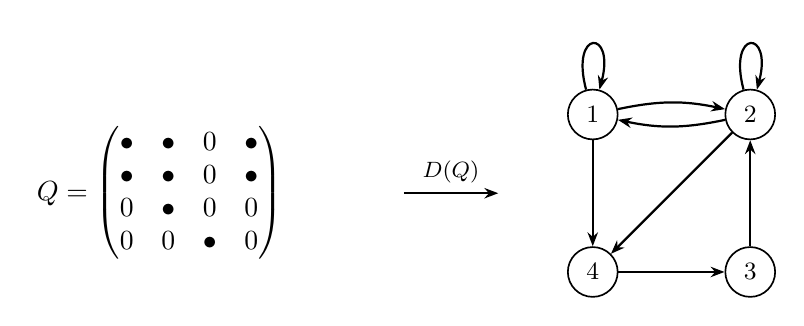
\begin{tikzpicture}[
  v/.style={circle, draw=black, line width=0.6pt, inner sep=1.2pt,
            minimum size=18pt, font=\small},
  arr/.style={-{Stealth[length=5pt]}, line width=0.8pt, draw=black},
]
% Matrix on the left
\node (mat) at (-2.5, 0) {$Q = \begin{pmatrix}
\bullet & \bullet & 0 & \bullet \\
\bullet & \bullet & 0 & \bullet \\
0 & \bullet & 0 & 0 \\
0 & 0 & \bullet & 0
\end{pmatrix}$};

% Arrow from matrix to digraph
\draw[-{Stealth[length=5pt]}, thick] (0.6, 0) -- (1.8, 0)
  node[midway, above, font=\footnotesize] {$D(Q)$};

% Digraph on the right (square layout, centered)
\node[v] (1) at (3.0, 1.0)  {1};
\node[v] (2) at (5.0, 1.0)  {2};
\node[v] (3) at (5.0, -1.0) {3};
\node[v] (4) at (3.0, -1.0) {4};

\draw[arr, loop above, looseness=8, min distance=8mm] (1) to (1);
\draw[arr, loop above, looseness=8, min distance=8mm] (2) to (2);
\draw[arr, bend left=12] (1) to (2);
\draw[arr, bend left=12] (2) to (1);
\draw[arr] (1) to (4);
\draw[arr] (2) to (4);
\draw[arr] (3) to (2);
\draw[arr] (4) to (3);
\end{tikzpicture}
\caption{A $4 \times 4$ upper Hessenberg matrix ($\bullet$ = nonzero) and its
support digraph $D(Q)$. Each nonzero entry $Q_{ij}$ becomes a directed arc
$i \to j$.}
\label{fig:intro-example}
\end{figure}
\FloatBarrier

\begin{definition}[Sign-equivalence]\label{def:sign}
\leanmargin{SignEquiv}{Matrix/SignEquivalence.lean\#L71}
Two matrices $Q, Q' \in \R^{n \times n}$ are \emph{sign-equivalent},
written $Q \simeq_{\mathrm{sign}} Q'$, if $Q' = D_L\, Q\, D_R$ for some
\emph{signature matrices} $D_L, D_R$ --- diagonal matrices whose diagonal
entries are all $\pm 1$.
\end{definition}

\begin{corollary}[Sign-invariance of the support digraph]\label{cor:sign-support}
\leanmargin{supportDigraph\_eq\_of\_signEquiv}{Matrix/SignEquivalence.lean\#L184}
Sign-equivalent matrices have identical zero / non-zero patterns; hence
$D(Q) = D(Q')$ whenever $Q \simeq_{\mathrm{sign}} Q'$.
\end{corollary}

\begin{definition}[Givens rotation, ordered Givens product]\label{def:givens}
\leanmargintwo{givensRotation}{Matrix/Givens/Rotation.lean\#L67}{givensProduct}{Matrix/Givens/Product.lean\#L69}
For $k \in \{0, \dots, n-2\}$ and $\theta \in \R$, the \emph{Givens rotation}
$G_k(\theta) \in \R^{n \times n}$ is the identity with the $2 \times 2$
block at rows / columns $(k, k{+}1)$ replaced by
$\bigl[\begin{smallmatrix}\cos\theta & -\sin\theta\\ \sin\theta & \cos\theta\end{smallmatrix}\bigr]$.
The \emph{ordered Givens product} of an angle vector $\theta = (\theta_0,
\dots, \theta_{n-2})$ is
\[
  Q_n(\theta) \;\defeq\; G_0(\theta_0)\, G_1(\theta_1)\,\cdots\,G_{n-2}(\theta_{n-2}).
\]
The product $Q_n(\theta)$ is always orthogonal upper Hessenberg, and its
$(k{+}1, k)$ subdiagonal entry equals $\sin\theta_k$.
\end{definition}

The angle vector is called \emph{unreduced} if every $\sin\theta_k$ is
non-zero; equivalently, every subdiagonal entry of $Q_n(\theta)$ is
non-zero. We write $\Theta_n$ for the set of such unreduced angle vectors.

\begin{definition}[Active set, combinatorial digraph]\label{def:active-set}
\leanmargintwo{ActiveSet}{ActiveSet.lean\#L70}{digraph}{ActiveSet.lean\#L281}
An \emph{active set} is any subset $S \subseteq [n-1]$. From $S$ we derive
\[
  R(S) \;\defeq\; \{1\} \cup \{k+1 : k \in S\}, \qquad
  C(S) \;\defeq\; S \cup \{n\}
\]
(\emph{active rows} / \emph{active columns}), and the \emph{combinatorial
digraph} $D_n(S)$ on $[n]$, whose arcs are of two kinds: \emph{spine} arcs
$j+1 \to j$ for $1 \le j \le n-1$, and \emph{overlay} arcs $i \to j$ whenever
$i \in R(S)$, $j \in C(S)$, and $i \le j$. This construction uses the set $S$
alone; no matrix or angle vector enters.

The \emph{active set of an angle vector} $\theta \in \Theta_n$ is
\[
  S(\theta) \;\defeq\; \bigl\{\, k+1 \,:\, k \in \{0, \dots, n-2\},\ \cos\theta_k \ne 0\,\bigr\} \;\subseteq\; [n-1],
\]
the subset to which $D_n$ is applied on the matrix side.
\end{definition}

\begin{example}[$n = 6$, $S = \{2, 4\}$ — anatomy of $D_6(\{2,4\})$]\label{ex:D6S24}
\leanmargin{example\_D6\_S24}{PaperExamples.lean\#L67}
The angle vector $\theta = (\pi/2, \pi/4, \pi/2, \pi/4, \pi/2)$ produces
$\cos\theta_k \ne 0$ exactly for $k \in \{1, 3\}$, hence
$S = \{2, 4\}$. The active rows and columns are
\[
  R = \{1, 3, 5\}, \qquad C = \{2, 4, 6\},
\]
and the resulting digraph $D_6(\{2, 4\})$ is depicted in
Figure~\ref{fig:digraph-anatomy}: the spine cycle in solid black and the
overlay arcs as dashed blue edges from $R$ to $C$. Here $R \cap C =
\emptyset$, so $D_6(\{2, 4\})$ has no self-loops.
\end{example}

\begin{figure}[htbp]
\centering
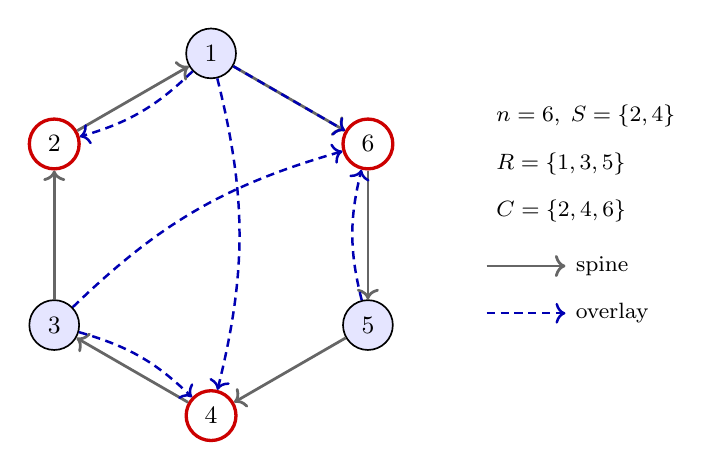
\begin{tikzpicture}[
  v/.style={circle, draw=black, line width=0.6pt, inner sep=1.2pt,
            minimum size=18pt, font=\small},
  spine/.style={->, line width=1.0pt, draw=black!60},
  over/.style={->, line width=0.9pt, draw=blue!70!black, densely dashed},
  Rnode/.style={fill=blue!10},
  Cnode/.style={draw=red!80!black, line width=1.2pt},
  RCnode/.style={fill=blue!10, draw=red!80!black, line width=1.2pt}
]
% n=6, S={2,4}
\def\radius{2.3}
\node[v,Rnode]  (1) at (90:\radius)  {1};
\node[v,Cnode]  (6) at (30:\radius)  {6};
\node[v,Rnode]  (5) at (-30:\radius) {5};
\node[v,Cnode]  (4) at (-90:\radius) {4};
\node[v,Rnode]  (3) at (-150:\radius){3};
\node[v,Cnode]  (2) at (150:\radius) {2};

% Spine (Hamilton cycle)
\draw[spine] (1) -- (6) node[midway, above right, font=\scriptsize, black!60] {};
\draw[spine] (6) -- (5);
\draw[spine] (5) -- (4);
\draw[spine] (4) -- (3);
\draw[spine] (3) -- (2);
\draw[spine] (2) -- (1);

% Overlay arcs: i in R={1,3,5}, j in C={2,4,6}, i <= j
\draw[over, bend left=14] (1) to (2);
\draw[over, bend left=14] (1) to (4);
\draw[over] (1) to (6);
\draw[over, bend left=14] (3) to (4);
\draw[over, bend left=14] (3) to (6);
\draw[over, bend left=14] (5) to (6);

% Legend
\node[anchor=west, font=\footnotesize] at (3.5, 1.5) {$n = 6,\; S = \{2, 4\}$};
\node[anchor=west, font=\footnotesize] at (3.5, 0.9) {$R = \{1, 3, 5\}$};
\node[anchor=west, font=\footnotesize] at (3.5, 0.3) {$C = \{2, 4, 6\}$};
\draw[spine] (3.5, -0.4) -- (4.5, -0.4)
  node[right, font=\footnotesize] {spine};
\draw[over] (3.5, -1.0) -- (4.5, -1.0)
  node[right, font=\footnotesize] {overlay};
\end{tikzpicture}
\caption{Anatomy of $D_6(\{2,4\})$. Solid arrows form the directed Hamilton
cycle (spine). Dashed blue arrows are the overlay arcs from active rows
$R = \{1,3,5\}$ (blue fill) to active columns $C = \{2,4,6\}$ (red outline).
Self-loops occur exactly at vertices in $R \cap C$; here $R \cap C =
\emptyset$, so $D_6(\{2,4\})$ is loopless.}
\label{fig:digraph-anatomy}
\end{figure}
\FloatBarrier

\begin{theorem}[Universality]\label{thm:universality}
\leanmargin{exists\_givensFactorization}{Matrix/Givens/Factorization.lean\#L840}
Every unreduced $Q \in \mathcal{H}_n$ is sign-equivalent to a canonical
Givens product: there exists $\theta \in \Theta_n$ with
$Q \simeq_{\mathrm{sign}} Q_n(\theta)$.
\end{theorem}

\begin{proof}[Proof sketch]
Induction on $n$. Right-multiply $Q$ by the transpose of a Givens factor
chosen to clear the last row to $e_n^\top$; orthogonality forces the last
column to $e_n$ as well, so the principal $(n{-}1) \times (n{-}1)$ corner
is itself orthogonal upper Hessenberg, and the induction hypothesis
applies. The accumulated sign discrepancies along the inductive peel-off
are absorbed into the diagonal $D_L, D_R$ of the sign-equivalence
relation.
\end{proof}

\begin{theorem}[Bridge]\label{thm:bridge}
\leanmargin{digraph\_model}{Realization/DigraphModel.lean\#L150}
For every $\theta \in \Theta_n$, the matrix support agrees with the
combinatorial digraph:
\[
  D\bigl(Q_n(\theta)\bigr) \;=\; D_n\bigl(S(\theta)\bigr).
\]
\end{theorem}

\begin{proof}[Proof sketch]
Two inclusions, both stated entry-wise on $Q_n(\theta)_{ij}$. The
subdiagonal entries are $\sin\theta_{j} \ne 0$ by the unreduced
hypothesis, exhibiting all spine arcs. For an upper-triangular entry
$i \le j$, a row / column-vanishing analysis on the Givens product shows
that $Q_n(\theta)_{ij} \ne 0$ iff $\cos\theta_{i-1} \ne 0$ and
$\cos\theta_{j} \ne 0$, which by definition of $S(\theta)$ is exactly the
overlay condition $i \in R(S(\theta))$, $j \in C(S(\theta))$.
\end{proof}

The bridge can be read off concretely from the matrix support pattern.
Returning to the running example $S = \{2, 4\}$ of
Example~\ref{ex:D6S24}, Figure~\ref{fig:matrix_pattern} highlights the
two kinds of nonzero entries promised by the theorem: the spine entries
$(j+1, j)$ on the subdiagonal (open circles), and the overlay entries at
positions $(i, j)$ with $i \in R$, $j \in C$, $i \le j$ (solid dots at
the row-column intersections).

\begin{figure}[htbp]
\centering
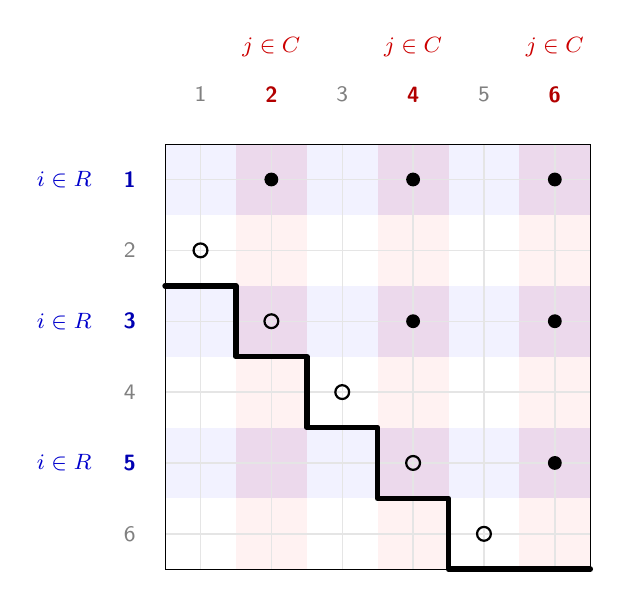
\begin{tikzpicture}[
    scale=0.9,
    grid line/.style={draw=gray!20, line width=0.5pt},
    hessenberg line/.style={draw=black, line width=2pt, line cap=round, line join=round},
    row band/.style={fill=blue!5},
    col band/.style={fill=red!5},
    cross cell/.style={fill=violet!15},
    subdiag node/.style={circle, draw=black, thick, inner sep=0pt, minimum size=5pt},
    entry node/.style={circle, fill=black, inner sep=0pt, minimum size=5pt}
]
\def\n{6}
\def\Rlist{1,3,5}
\def\Clist{2,4,6}

% Background bands
\foreach \r in \Rlist {
    \fill[row band] (0.5, -\r+0.5) rectangle (\n.5, -\r-0.5);
    \node[anchor=east, blue!80!black, font=\footnotesize] at (-0.4, -\r) {$i \in R$};
}
\foreach \c in \Clist {
    \fill[col band] (\c-0.5, -0.5) rectangle (\c+0.5, -\n.5);
    \node[anchor=south, red!80!black, font=\footnotesize] at (\c, 0.6) {$j \in C$};
}

% Intersection cells
\foreach \r in \Rlist {
    \foreach \c in \Clist {
        \fill[cross cell] (\c-0.5, -\r+0.5) rectangle (\c+0.5, -\r-0.5);
    }
}

% Labels
\foreach \k in {1,...,\n} {
    \let\rstyle\relax \def\rcolor{gray}
    \foreach \x in \Rlist { \ifnum\x=\k \global\def\rstyle{\bfseries} \global\def\rcolor{blue!70!black} \fi }
    \node[font=\sffamily\footnotesize\rstyle, color=\rcolor] at (0, -\k) {\k};
    \let\cstyle\relax \def\ccolor{gray}
    \foreach \x in \Clist { \ifnum\x=\k \global\def\cstyle{\bfseries} \global\def\ccolor{red!70!black} \fi }
    \node[font=\sffamily\footnotesize\cstyle, color=\ccolor] at (\k, 0.2) {\k};
}

% Grid
\draw[grid line] (0.5, -0.5) grid (\n.5, -\n.5);
\draw[black, thin] (0.5, -0.5) rectangle (\n.5, -\n.5);

% Hessenberg barrier
\draw[hessenberg line]
    (0.5, -2.5)
    \foreach \k in {1,...,4} {
        -- (\k.5, -\k.5-1)
        -- (\k.5, -\k.5-2)
    }
    -- (6.5, -6.5);

% Nonzeros
\foreach \k in {1,...,5} {
    \node[subdiag node] at (\k, -\k-1) {};
}
\foreach \r in \Rlist {
    \foreach \c in \Clist {
        \pgfmathparse{int(\r<=\c)}
        \ifnum\pgfmathresult=1
            \node[entry node] at (\c, -\r) {};
        \fi
    }
}
\end{tikzpicture}
\caption{Support pattern of $Q_6(\{2, 4\})$, the matrix-side counterpart of
Figure~\ref{fig:digraph-anatomy}. The thick boundary marks the upper
Hessenberg band; open circles ($\circ$) are the mandatory subdiagonal
spine entries; solid dots ($\bullet$) are overlay nonzeros at the
intersections (purple) of active rows (blue) and active columns (red).
The Bridge theorem says these are exactly the nonzero entries of any
unreduced $Q_n(\theta)$ with $S(\theta) = \{2, 4\}$.}
\label{fig:matrix_pattern}
\end{figure}
\FloatBarrier

\begin{example}[$n = 5$, $S = \{2\}$]\label{ex:D5S2}
\leanmargin{example\_D5\_S2}{PaperExamples.lean\#L131}
The angle vector $\theta = (\pi/2, \pi/4, \pi/2, \pi/2)$ gives:
\[
Q = \begin{pmatrix}
0 & \tfrac{1}{\sqrt{2}} & 0 & 0 & \tfrac{1}{\sqrt{2}} \\
-1 & 0 & 0 & 0 & 0 \\
0 & -\tfrac{1}{\sqrt{2}} & 0 & 0 & \tfrac{1}{\sqrt{2}} \\
0 & 0 & -1 & 0 & 0 \\
0 & 0 & 0 & -1 & 0
\end{pmatrix},
\qquad
A = \begin{pmatrix}
0 & 1 & 0 & 0 & 1 \\
1 & 0 & 0 & 0 & 0 \\
0 & 1 & 0 & 0 & 1 \\
0 & 0 & 1 & 0 & 0 \\
0 & 0 & 0 & 1 & 0
\end{pmatrix}.
\]
The Hamilton cycle is $1 \to 5 \to 4 \to 3 \to 2 \to 1$. Since
$R = \{1, 3\}$ and $C = \{2, 5\}$ are disjoint, the digraph is loopless
(Figure~\ref{fig:D5S2}); $A$ is exactly the support pattern predicted by
Theorem~\ref{thm:bridge}.
\end{example}

\begin{figure}[htbp]
\centering
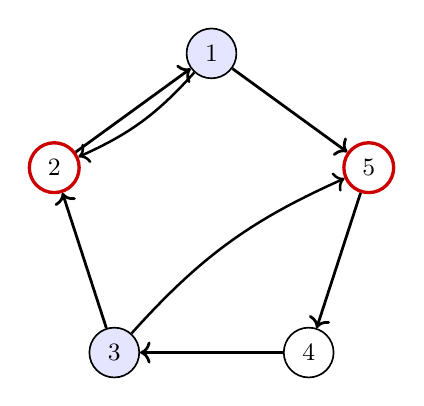
\begin{tikzpicture}[
  v/.style={circle, draw=black, line width=0.6pt, inner sep=1.2pt,
            minimum size=18pt, font=\small},
  cyc/.style={->, line width=1.0pt, draw=black},
  extra/.style={->, line width=0.9pt, draw=black},
  Rnode/.style={fill=blue!10},
  Cnode/.style={draw=red!80!black, line width=1.2pt}
]
\node[v,Rnode] (1) at ( 90:2.1) {1};
\node[v,Cnode] (5) at ( 18:2.1) {5};
\node[v]       (4) at (-54:2.1) {4};
\node[v,Rnode] (3) at (-126:2.1) {3};
\node[v,Cnode] (2) at (162:2.1) {2};

\draw[cyc] (1) -- (5);
\draw[cyc] (5) -- (4);
\draw[cyc] (4) -- (3);
\draw[cyc] (3) -- (2);
\draw[cyc] (2) -- (1);

\draw[extra, bend left=12] (1) to (2);
\draw[extra, bend left=12] (3) to (5);
\end{tikzpicture}
\caption{The loopless support digraph $D_5(\{2\})$. Active rows $R = \{1,3\}$
(blue fill) and active columns $C = \{2,5\}$ (red outline) are disjoint.}
\label{fig:D5S2}
\end{figure}
\FloatBarrier

\begin{theorem}[Rigidity]\label{thm:rigid}
\leanmargin{rigid}{Combinatorial/Rigidity.lean\#L331}
Let $S, S' \subseteq [n-1]$ with $|S|, |S'| \ge 2$. If $D_n(S) \cong D_n(S')$
as digraphs, then $S = S'$.
\end{theorem}

\begin{proof}[Proof sketch]
The key combinatorial fact is the \emph{cut lemma}: in $D_n(S)$, the only
arc from $\{k{+}1, \dots, n\}$ to $\{1, \dots, k\}$ is the spine arc
$k{+}1 \to k$. This forces every isomorphism to fix the unique directed
Hamilton cycle $1 \to n \to n{-}1 \to \cdots \to 2 \to 1$. A pigeonhole
argument on the cut, combined with degree analysis at the
maximum-in-degree vertex (which is $n$ when $|S| \ge 2$), forces the
isomorphism to fix $n$, after which a downward induction along the cycle
forces the identity. The case $|S| = 1$ is the only failure: the cyclic
rotation $\rho^t$ exhibits $D_n(\{t\}) \cong D_n(\{n - t\})$, with no
further coincidences.
\end{proof}

\begin{example}[$n = 5$, $S = \{1, 3\}$]\label{ex:D5S13}
\leanmargin{example\_D5\_S13}{PaperExamples.lean\#L186}
A two-element example illustrating Theorem~\ref{thm:rigid}: any
$D_5(S')$ isomorphic to $D_5(\{1,3\})$ must have $S' = \{1, 3\}$. The
angle vector $\theta = (\pi/4, \pi/2, \pi/4, \pi/2)$ gives:
\[
Q = \begin{pmatrix}
\tfrac{1}{\sqrt{2}} & 0 & \tfrac{1}{2} & 0 & \tfrac{1}{2} \\
-\tfrac{1}{\sqrt{2}} & 0 & \tfrac{1}{2} & 0 & \tfrac{1}{2} \\
0 & -1 & 0 & 0 & 0 \\
0 & 0 & -\tfrac{1}{\sqrt{2}} & 0 & \tfrac{1}{\sqrt{2}} \\
0 & 0 & 0 & -1 & 0
\end{pmatrix},
\qquad
A = \begin{pmatrix}
1 & 0 & 1 & 0 & 1 \\
1 & 0 & 1 & 0 & 1 \\
0 & 1 & 0 & 0 & 0 \\
0 & 0 & 1 & 0 & 1 \\
0 & 0 & 0 & 1 & 0
\end{pmatrix}.
\]
Here $R \cap C = \{1\}$, so there is exactly one self-loop at vertex~$1$
(Figure~\ref{fig:D5S13}).
\end{example}

\begin{figure}[htbp]
\centering
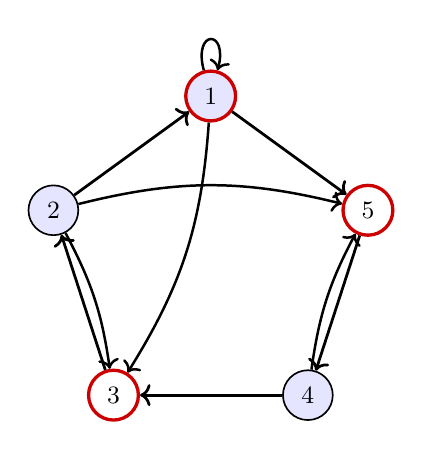
\begin{tikzpicture}[
  v/.style={circle, draw=black, line width=0.6pt, inner sep=1.2pt,
            minimum size=18pt, font=\small},
  cyc/.style={->, line width=1.0pt, draw=black},
  extra/.style={->, line width=0.9pt, draw=black},
  Rnode/.style={fill=blue!10},
  Cnode/.style={draw=red!80!black, line width=1.2pt},
  RCnode/.style={fill=blue!10, draw=red!80!black, line width=1.2pt}
]
\node[v,RCnode] (1) at ( 90:2.1) {1};
\node[v,Cnode]  (5) at ( 18:2.1) {5};
\node[v,Rnode]  (4) at (-54:2.1) {4};
\node[v,Cnode]  (3) at (-126:2.1) {3};
\node[v,Rnode]  (2) at (162:2.1) {2};

\draw[cyc] (1) -- (5);
\draw[cyc] (5) -- (4);
\draw[cyc] (4) -- (3);
\draw[cyc] (3) -- (2);
\draw[cyc] (2) -- (1);

\draw[extra, loop above] (1) to (1);
\draw[extra, bend left=14] (1) to (3);
\draw[extra, bend left=10] (2) to (3);
\draw[extra, bend left=14] (2) to (5);
\draw[extra, bend left=10] (4) to (5);
\end{tikzpicture}
\caption{The support digraph $D_5(\{1,3\})$. Since $R \cap C = \{1\}$, there
is exactly one self-loop at vertex~$1$.}
\label{fig:D5S13}
\end{figure}
\FloatBarrier

\begin{theorem}[Classification]\label{thm:classification}
\leanmargin{classification}{Classification.lean\#L54}
Fix $n \ge 2$. The classification of support digraphs of unreduced
orthogonal upper Hessenberg matrices is the conjunction:
\begin{enumerate}[label=\textup{(\arabic*)}]
\item \textup{(realizability)} every $S \subseteq [n-1]$ is of the form
  $S(\theta)$ for some $\theta \in \Theta_n$;
\item \textup{(bridge)} for every $\theta$, the support of $Q_n(\theta)$
  equals $D_n(S(\theta))$;
\item \textup{(rigidity)} for every $S, S'$ with $|S|, |S'| \ge 2$,
  $D_n(S) \cong D_n(S') \Rightarrow S = S'$.
\end{enumerate}
\end{theorem}

The classification declaration is a one-line term-level packaging of three
independently-proved components; it adds no mathematical content and exists
only so the paper has a single Lean handle to cite. Realizability is
witnessed by the explicit angle choice $\theta_k = \pi/4$ if $k+1 \in S$,
$\theta_k = \pi/2$ otherwise; this gives $\sin \theta_k \ne 0$ always and
$\cos\theta_k \ne 0$ exactly on $S$.


\begin{theorem}[Connected count]\label{thm:count}
\leanmargin{card\_isoClasses\_quot}{Combinatorial/ClassCount.lean\#L268}
For $n \ge 2$, the number of non-isomorphic weakly connected support
digraphs of $n \times n$ unreduced orthogonal upper Hessenberg matrices is
\[
  N_n \;=\; 2^{\,n-1} \;-\; \Big\lfloor \tfrac{n-1}{2} \Big\rfloor.
\]
\end{theorem}

\begin{theorem}[Loopless count]\label{thm:count-loopless}
\leanmargin{card\_looplessClasses\_quot}{Combinatorial/ClassCount.lean\#L526}
For $n \ge 3$, the number of non-isomorphic loopless connected support
digraphs is
\[
  N_n^{\mathrm{loopless}} \;=\; F_{n-1} \;-\; \Big\lfloor \tfrac{n-3}{2} \Big\rfloor,
\]
where $F_k$ is the $k$-th Fibonacci number ($F_0 = 0$, $F_1 = 1$).
\end{theorem}

\begin{proof}[Proof sketch \textup{(both counts)}]
Both counts follow the same template: \emph{labeled} configurations are
subsets $S \subseteq [n-1]$ (resp.\ $S \subseteq \{2, \dots, n-2\}$ with
no consecutive elements, the loopless characterisation). The number of
labeled configurations is $2^{n-1}$ (resp.\ $F_{n-1}$ via the standard
Fibonacci-counts-binary-strings bijection). Subsets with $|S| \ge 2$ are
rigid (Theorem~\ref{thm:rigid}), so each is its own isomorphism class.
The empty subset is rigid alone. The $|S| = 1$ subsets pair up under
$\{t, n-t\}$, contributing $\lceil(n-1)/2\rceil$ (resp.\
$\lceil(n-3)/2\rceil$) classes.
\end{proof}



\appendix
% !TEX root = ../main_hessenberg.tex
\begin{comment}
\section{Compression as evidence of content}\label{sec:compression}

The criteria of \S\ref{sec:methodology} are internal: a green build,
and an apex signature that reads as the paper sentence. Both are
judgments the authors pass on their own artifact. This section adds
an external one. Aksenov, Bodnia, Freedman, and
Mulligan~\cite{aksenov2026compressionneedmodelingmathematics} take
compression as the measurable difference between mathematics and
mere formal text, and calibrate this on Mathlib: unfolding genuine
mathematics expands the source by many orders of magnitude, which
formal text restating its premises does not. We state their measure,
compute it for our development, and report where the development
lands.

\begin{definition}[Compression metrics,
{\cite[\S3]{aksenov2026compressionneedmodelingmathematics}}]\label{def:abfm}
\leanmarginLean{Util.Compression}{Util/Compression.lean}
Let $G$ be the directed graph whose vertices are the declarations of
a Lean development plus a synthetic vertex $\mathsf{Sort}$, with an
edge $u \to v$ of weight $w$ when the elaborated term of $u$ refers
to $v$ exactly $w$ times; declarations of the Lean core library and
$\mathsf{Sort}$ are \emph{primitive}. The \emph{wrapped length} of
$u$ is the number of tokens in its Lean source. Its \emph{unwrapped
length} is $|u|_G = \sum_i w_i \, |v_i|_G$ over the edges
$u \to v_i$, with $|u|_G = 1$ for primitives. Its \emph{depth} is
the length of the longest path in $G$ from $u$ to a primitive.
\end{definition}

Wrapped length is the cost of stating $u$ with the whole library at
hand; unwrapped length is the cost of stating it from primitives
alone. The ratio between the two measures the compression that the
intervening definitions buy, and depth counts how many layers of
definitions that compression is spread across.

We compute the three quantities for the thirteen public targets of
\texttt{HessenbergDigraphs} with a program written in Lean itself,
invoked as \texttt{lake exe hessenberg-compression}. The program is a
transcription of Definition~\ref{def:abfm}: it loads the compiled
library at runtime, collects the weighted reference multiset of each
elaborated term by structural recursion over the term (the
\texttt{collectElems} traversal of Aksenov et al.\ \S3.1), and evaluates
$|u|_G$ and depth by memoised recursion over $G$. Working inside Lean
gives the program the elaborated terms exactly as the kernel checked
them, rather than a reconstruction from printed output. Three
implementation choices on points that their description leaves
open (the tokenizer behind wrapped length, the references of
declarations that have a type but no term, such as inductive types
and their recursors, and cycle handling) are documented in the
source. The results appear in Table~\ref{tab:compression}.

\begin{table}[ht]
\centering
\renewcommand{\arraystretch}{1.05}
\begin{tabular}{@{}lrrr@{}}
\toprule
\textbf{Declaration} & \textbf{Wrapped} & \textbf{Unwrapped} & \textbf{Depth} \\
\midrule
\texttt{classification}              &     93 & $2.39 \times 10^{44}$ & 138 \\
\texttt{completeness}                &     61 & $2.38 \times 10^{44}$ & 137 \\
\texttt{digraph\_model}              &    123 & $4.95 \times 10^{41}$ & 114 \\
\texttt{exists\_givensFactorization} &    368 & $2.81 \times 10^{47}$ & 147 \\
\texttt{rigid}                       &  1\,201 & $2.44 \times 10^{12}$ &  28 \\
\texttt{singleton\_iso}              &    139 & $2.05 \times 10^{11}$ &  24 \\
\texttt{singleton\_iso\_unique}      &  1\,052 & $1.83 \times 10^{12}$ &  28 \\
\texttt{loopless\_iff}               &    566 & $1.01 \times 10^{8}$  &  21 \\
\texttt{count\_formula}              &     67 & $4.30 \times 10^{9}$  &  21 \\
\texttt{count\_loopless\_formula}    &     97 & $193\,677$            &   4 \\
\texttt{Arc}                         &     75 & $8$                   &   2 \\
\texttt{activeSet}                   &    100 & $1.01 \times 10^{37}$ & 101 \\
\texttt{givensProduct}               &     51 & $1.35 \times 10^{37}$ & 102 \\
\bottomrule
\end{tabular}
\caption{Compression metrics (wrapped, unwrapped, depth) of
Definition~\ref{def:abfm} for the thirteen public targets of
\texttt{HessenbergDigraphs}, computed by
\texttt{lake exe hessenberg-compression}.}
\label{tab:compression}
\end{table}

The four apex-level theorems and the foundation definition
\texttt{activeSet} have unwrapped lengths between $10^{37}$ and
$10^{47}$ and depths above $100$. This crosses the threshold by which
Aksenov et al.\ separate genuine hierarchical compression from mere
syntactic restatement, placing the project within the substantive-content
region of Mathlib: below their reported maximum of $10^{104}$, but
unambiguously inside the compression regime. The two enumeration
formulae and the singleton isomorphism sit in the
$10^{8}$--$10^{12}$ range at depths $20$--$28$, corresponding to
proofs that form a structural-lemma chain built on top of arithmetic
identities. \texttt{count\_loopless\_formula} is the smallest
target, at depth $4$ and unwrapped length $193\,677$: the proof is a
single closed-form arithmetic identity, which the metric reads off
directly.

This answers the question that the choice of a marshmallow invites:
a deliberately elementary problem has not left the artifact empty.
The internal criterion of \S\ref{sec:methodology} says the code reads
as mathematics; the measurement here says the case study of
\S\ref{sec:example} measures as mathematics.
\end{comment}

% !TEX root = ../main_hessenberg.tex

\begin{comment}
\section{Code statistics}\label{sec:appendix-stats}

\begin{center}
\renewcommand{\arraystretch}{1.2}
\begin{tabular}{@{}lr@{}}
\toprule
\textbf{Metric} & \textbf{Value} \\
\midrule
Total lines of Lean code & 2\,227 \\
Definitions (\texttt{def}/\texttt{noncomputable def}) & 19 \\
Theorems and lemmas & 48 \\
\texttt{sorry} count & 0 \\
Axioms (via \texttt{\#print axioms}) & 3 \\
\quad\texttt{propext} & \\
\quad\texttt{Classical.choice} & \\
\quad\texttt{Quot.sound} & \\
\texttt{maxHeartbeats} overrides & 2 (both 800\,000) \\
\bottomrule
\end{tabular}
\end{center}

The two \texttt{maxHeartbeats} overrides apply to \texttt{singleton\_iso} and
\texttt{singleton\_iso\_unique}, both involving extensive modular arithmetic
case analysis. All other proofs compile within the default heartbeat limit.

The source code is available at
\url{https://github.com/[repository]}.
\end{comment}


% =====================================================================
\bibliographystyle{alpha}
\bibliography{references}

\end{document}
